\subsubsection{Guidance method's questionnaire.}
\label{subsubsec:results_questionnaires_2}

As was for the blind users, the sighted user also answered the Guidance questionaire to give their thoughts about their experience as BVI users. This way is possible to compare their feelings of confort and safety and compare with the blind users. The Table \ref{tab:questionnaire_average} shows the score of both groups of each method and they are plotted in the Figure \ref{fig:barplot_sagat_avg_4_scene}.


\begin{table}[!htb]
\centering
\caption{Guidance method questionnaire average score grouped by participant.}
\label{tab:questionnaire_average}
\begin{tabular}{lllrrrrr}
\toprule
{} & Audio & \begin{tabular}[c]{@{}l@{}}Haptic\\ Belt\end{tabular} & \begin{tabular}[c]{@{}l@{}}Virtual\\ Cane\end{tabular} & Mixture & Visual Condition \\
Participant &       &                                                       &                                                        &         &                  \\
\midrule
001         &  0.75 &                                                  0.49 &                                                   0.57 &    0.69 &            Sight \\
001C        &  0.77 &                                                  0.54 &                                                   0.63 &    0.87 &            Blind \\
002C        &  0.86 &                                                  0.74 &                                                   0.54 &    0.93 &            Blind \\
003         &  0.76 &                                                  0.54 &                                                   0.54 &    0.78 &            Sight \\
003C        &  0.93 &                                                  0.57 &                                                   0.54 &    0.74 &            Blind \\
004         &  0.86 &                                                  0.60 &                                                   0.79 &    0.76 &            Sight \\
004C        &  0.88 &                                                  0.49 &                                                   0.40 &    0.73 &            Blind \\
005         &  0.61 &                                                  0.57 &                                                   0.75 &    0.84 &            Sight \\
\bottomrule
\end{tabular}
\end{table}



 The Figure \ref{fig:barplot_sagat_avg_4_scene} presents the average score of each group. It possible to see that both groups were pleased with the "Audio" and "Mixture" method. The difference lies in the preference between the "Haptic Belt" and "Virtual Cane". The blind users tend to prefer the first while the sighted users tend to prefer the last.

%\begin{figure}[!htb]
%    \centering
%    \begin{minipage}{\textwidth}
%        \centering
%        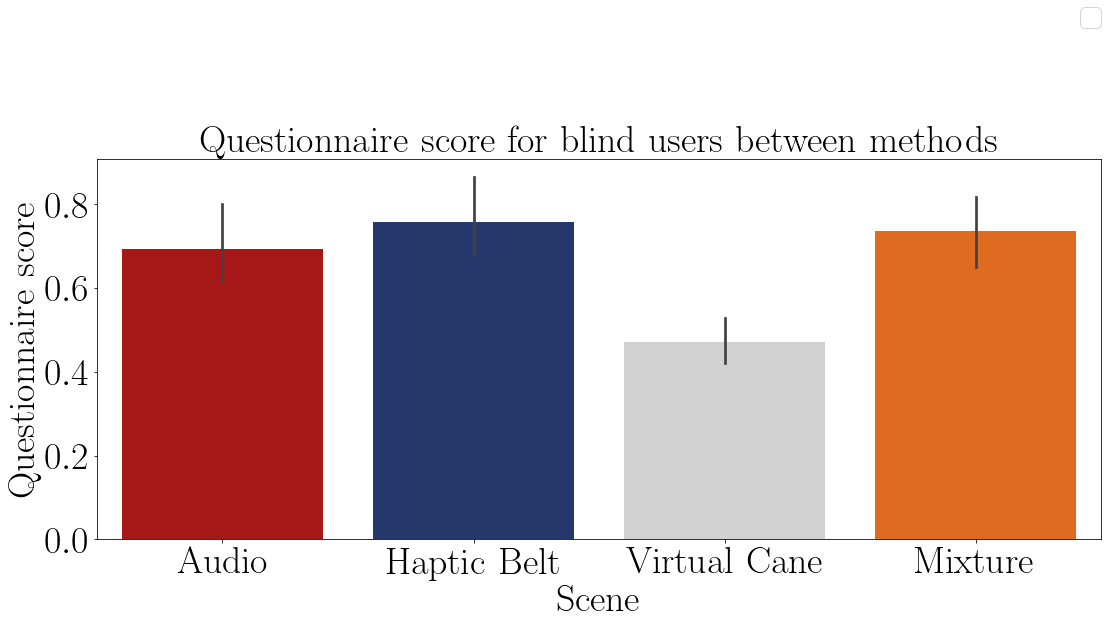
\includegraphics[width = 0.8\linewidth]{Resultados/Questionario/Figuras/png/barplot_questionnaire_scene_blind.png}
%        \caption{Barplot of the average questionaire score of the blind participants on each method.}
%        \label{fig:barplot_questionnaire_scene_blind_2}
%    \end{minipage}
%    \begin{minipage}{\textwidth}
%        \centering
%        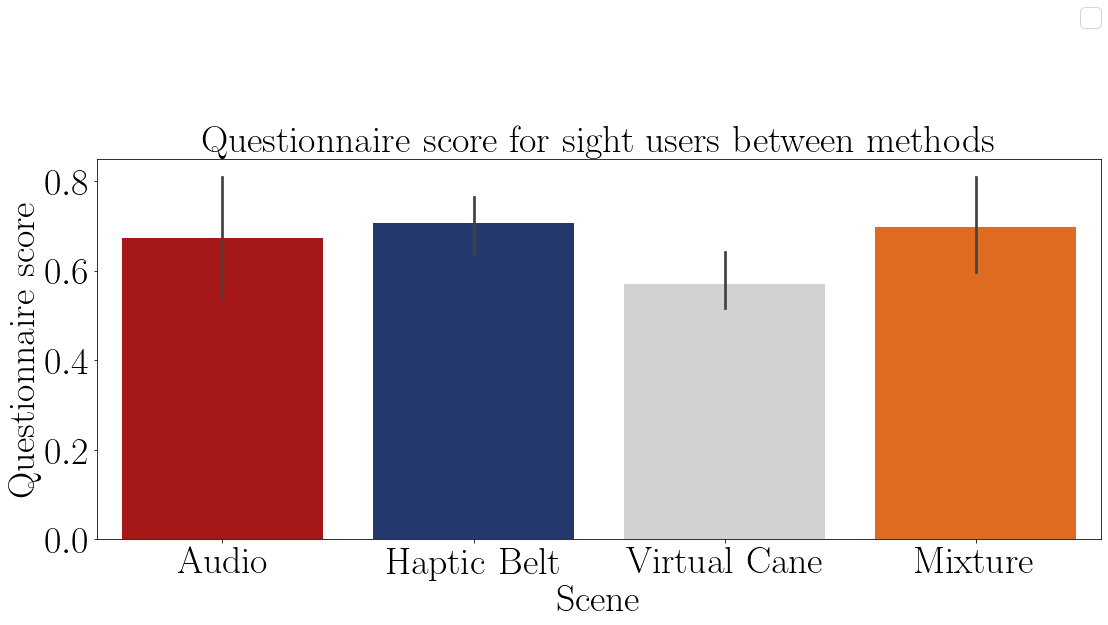
\includegraphics[width = 0.8\linewidth]{Resultados/Questionario/Figuras/png/barplot_questionnaire_scene_sight.png}
%        \caption{Barplot of the average questionaire score of the sighted participants on each method.}
%        \label{fig:barplot_questionnaire_scene_sight}
%    \end{minipage}
%\end{figure}
\begin{figure}[!htb]
    \centering
    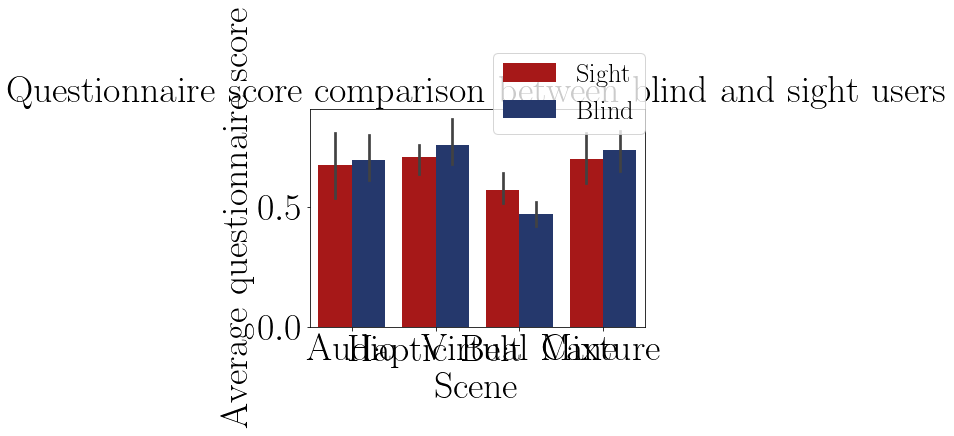
\includegraphics[width = 0.8\linewidth]{Resultados/Questionario/Figuras/png/barplot_questionnaire_scene.png}
    \caption{Barplot of the  average questionaire score of both participants on each method.}
    \label{fig:barplot_questionnaire_scene}
\end{figure}

The Figure \ref{fig:boxplot_questionnaire_scene} presents the scores distribution and it is posible to see that there is some similarity between the two groups, with the exception of the "Virtual Cane" method, which has a wider distributiuon for the sighted users. Also, it seems that the "Audio" and "Mixture" are similar inside the sighted users, as it was with the blind users..

\begin{figure}[!htb]
    \centering
    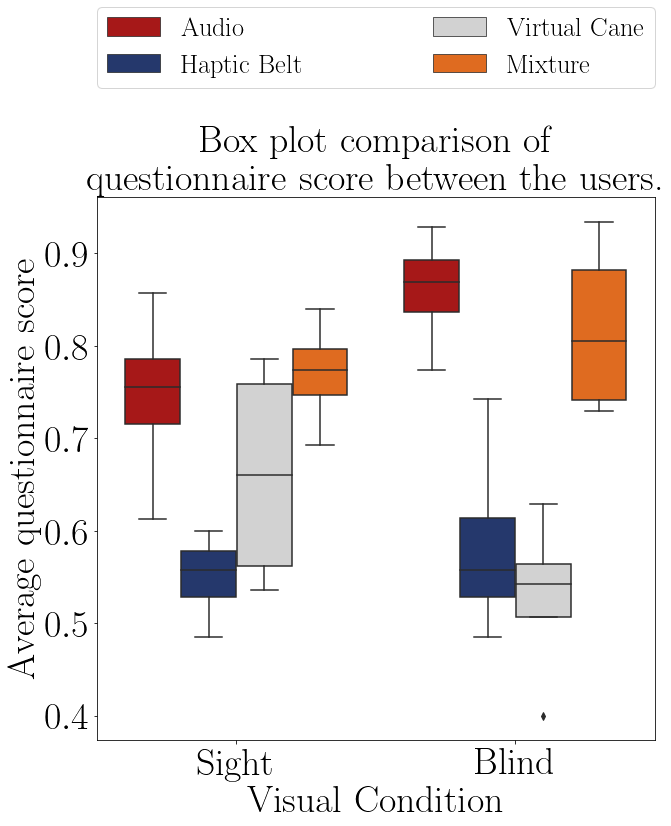
\includegraphics[width = 0.6\linewidth]{Resultados/Questionario/Figuras/png/boxplot_questionnaire_scene.png}
    \caption{Boxplot of the questionaire score of the the participants grouped by method.}
    \label{fig:boxplot_questionnaire_scene}
\end{figure}

The Table \ref{tab:questionnaire_average_group} show the the average questionnaire score on each method of both groups and it shows the same conclusion as the Figure \ref{fig:barplot_questionnaire_scene}, that the preference between the "Haptic Belt" and "Virtual Cane" is the only difference between the two groups.

Considering the most preferable and the less preferable of each group, the blind users are score their choices more intesiver than the sighted users. This may be an effect from their previous experience with the "Audio" method in previous events before the experiment and with haptic devices were something very, or almost, new. For the sighted users everything was new, so there scores were more consistent. This is posible to see in the average and standar deviation of these scores. For the blind users is 0.7 and 0.164 and for the sighted user is 0.682 and 0.100.


\begin{table}[!htb]
\centering
\caption{Guidance method questionnaire average score grouped by visual condition.}
\label{tab:questionnaire_average_group}
\begin{tabular}{lllll}
\toprule
{} &  Audio &  Haptic Belt &  Virtual Cane &  Mixture \\
Visual Condition &        &              &               &          \\
\midrule
Blind            &  0.693 &        0.757 &         0.471 &    0.735 \\
Sight            &  0.674 &        0.707 &         0.571 &    0.698 \\
\bottomrule
\end{tabular}
\end{table}



The Figures \ref{fig:qqplot_questionnaires_sight} and \ref{fig:residplot_questionnaires_sight} shows the distribution and variance of the Table \ref{tab:questionnaire_average}. These Figures shows that the data are normally distributed and that the methods have a similar variance.
The Table \ref{tab:blocanova_questionnaire_sight} shows the Anova test p-value of the questionnaire score of the "sight" sample. The p-values indicates that the method have influence on the score. Meaning that the participants had differents level os satisfaction about each method.


\begin{table}[!htb]
\centering
\caption{Anova p-value for the questionnaire score on each method for blinded users.}
\label{tab:blocanova_questionnaire_sight}
\begin{tabular}{lrrrrr}
\toprule
Source & P-Value \\
\midrule
Method & 0.016** \\
\bottomrule
\end{tabular}
\end{table}



\begin{figure}[!htb]
    \centering
    \begin{minipage}{0.45\textwidth}
        \centering
        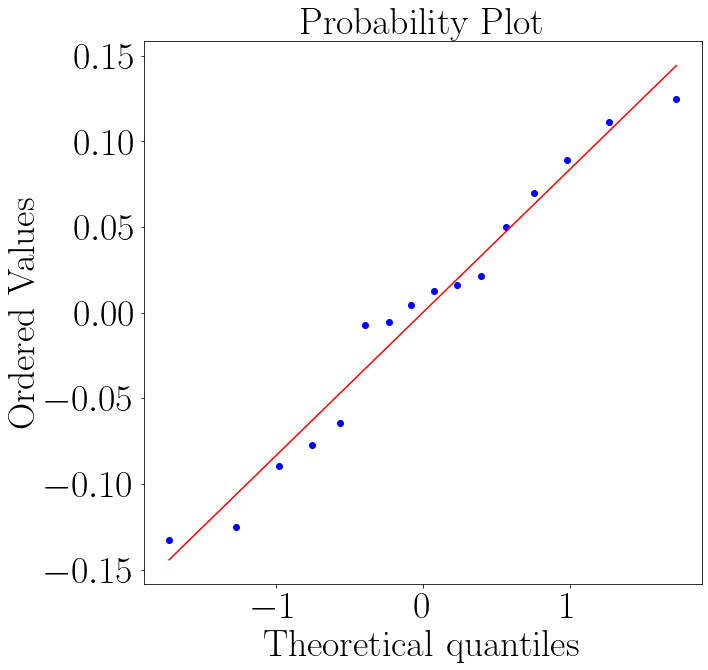
\includegraphics[width = 0.8\linewidth]{Resultados/Questionario/Figuras/png/qqplot_questionnaires_sight.png}
        \caption{QQ plot of the questionnaire score of the sighted participants on each method.}
        \label{fig:qqplot_questionnaires_sight}
    \end{minipage}
    \begin{minipage}{0.45\textwidth}
        \centering
        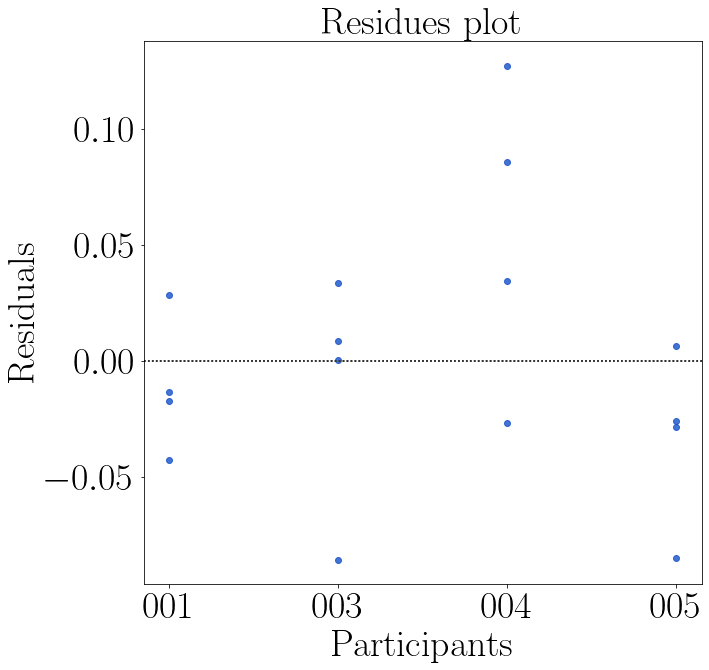
\includegraphics[width = 0.8\linewidth]{Resultados/Questionario/Figuras/png/residplot_questionnaires_sight.png}
        \caption{Residual plot of the questionnaire score the sighted participants on each method.}
        \label{fig:residplot_questionnaires_sight}
    \end{minipage}
\end{figure}

The Table \ref{tab:lsd_questionnaire_sight} presents the conclusion of a pairwise Fisher LSD test between all the guidance methods. The results are the same as the one for the "blind" users. That only the "Audio" and "Mixture" have the same statistically result and that there is a difference between the both "Haptic Belt" and "Virtual Cane".


\begin{table}[!htb]
\centering
\caption{Cross validation p-value for the questionnaire score on each method for blinded users.}
\label{tab:lsd_questionnaire_sight}
\begin{tabular}{rclr}
\toprule
      \multicolumn{3}{c}{Method} &                                           Analysis \\
\midrule
       Audio & $X$ & Haptic Belt &        $H_1 : \mu_{Audio} \ne \mu_{Haptic Belt}**$ \\
      Audio & $X$ & Virtual Cane &       $H_1 : \mu_{Audio} \ne \mu_{Virtual Cane}**$ \\
           Audio & $X$ & Mixture &                $H_0 : \mu_{Audio} = \mu_{Mixture}$ \\
Haptic Belt & $X$ & Virtual Cane & $H_1 : \mu_{Haptic Belt} \ne \mu_{Virtual Cane}**$ \\
     Haptic Belt & $X$ & Mixture &      $H_1 : \mu_{Haptic Belt} \ne \mu_{Mixture}**$ \\
    Virtual Cane & $X$ & Mixture &     $H_1 : \mu_{Virtual Cane} \ne \mu_{Mixture}**$ \\
\bottomrule
\end{tabular}
\end{table}



The LSD Table \ref{tab:lsd_questionnaire_sight} repeat the same conclusion of the blind participants, that only the "Audio" and "Mixture" are statistically the same. But that does not mean that both groups had the same opinion from the rest of the methods. As shown in the Figure \ref{fig:boxplot_questionnaire_scene}, the average sighted user rather use the "Virtual Cane" then the "Haptic Belt", despite that distribution being wider, hence more varied, meaning that this is hardly a consense between the users.

\FloatBarrier